\chapter{Spelling normalization}
In the sixteenth and seventeenth century, Dutch authors and printers didn't highly value the consistency of word spellings. This resulted in many different spelling variants of the same word coexisting. Because a topic modeling method only looks at the position of words and how they are distributed through the corpus, it sees different spellings of the same word as different words. For instance, \enquote{Jezus}, \enquote{Jesu} and \enquote{Iesus} are regarded as different words, as well as \enquote{bloed} and \enquote{bloet}. It is easy to understand that this biases the results of the topic modeling process. Therefore normalization of spelling is a crucial step that needs to be taken. Regarding the English language, quite some tools are available for converting historical texts to a standard spelling. For the Dutch language, options are limited, especially methods that are straightforward method and do not cost too much time. The tools that are available, come with both advantages and disadvantages. I have chosen to use two different methods to normalize the spelling of my corpus. After normalization with these two methods, I will perform topic modeling on the two different normalized versions of my corpus, as well on the unnormalized version of my corpus, e.g. the original texts. Hopefully the results of topic modeling will give more insight which version of the corpus is the most productive to work with. Below I discuss the two tools that I will use for spelling normalization. To illustrate the performance of both tools, I will show the normalized spelling versions of one particular song lyric\footnote{\texttt{id} = 186989.} later on. Here I show the original version of this song:

\begin{quote}
	Daar de gulde zon en maan\\
	En de mindre hemelvieren,\\
	Die het stargewelf vercieren,\\
	Gods geboden gadeslaan:\\
	Daar de felle noordewinden\\
	In het bruissend element\\
	Op die stem zig laten binden:\\
	Wie roept dat hy God niet kent?\\
	
	'T aards gezinde en dwaze rot\\
	Op het vroom geslagt verbolgen\\
	En geneigt zijn lust te volgen,\\
	Durft zig uiten, daar 's geen God.\\
	Welkers oordeel sta te vreezen\\
	Als het lighaam zinkt in 't graf.\\
	Want de ziel verliest haar wezen,\\
	Als wy leggen 't leven af.\\
	
	Aartsverraders schrikt, ziet toe\\
	Gods gedult, en hand te tergen.\\
	Voor zijn oog is geen verbergen.\\
	Vreest, vreest 's Hemels strenge roe!\\
	Eenmaal zal de dag genaken.\\
	(Is zijn wrake traag in 't gaan)\\
	Die u zal te schande maken,\\
	En door blixemvuur verslaan.
\end{quote}

\section{INL}
The first method I have used to modernize spelling is a tool built by Marijn Schraagen and Martijn van der Klis. The modernization is performed by querying all words in the corpus using the INT Lexicon Service\footnote{http://sk.taalbanknederlands.inl.nl/LexiconService/.} and replacing the words with the lemma resulting from the query. An important note is that the tool cannot be trained: the first result of the query in the Lexicon Service is always chosen as output, and this can not be manipulated. This means that it's hard to correct the mistakes that are made by the tool. In addition, all verbal words are normalized to the infinitive, which means that the difference between past and present forms disappears. After normalization with INL, the song mentioned above looks like this:

\begin{quote}
	Daar de gild zon en maan\\
	En de minder hemelvieren\\
	Die het stergewelf versieren\\
	Gods geboden gadeslaan :\\
	Daar de fel noordewinden\\
	In het bruissend element\\
	Op die stem zek laten binden :\\
	Wie roepen dat hei God niet ken ?\\
	
	'T aards gezinde en dwaas rot\\
	Op het vroom geslacht verbolgen\\
	En neigen zijn lust te volgen\\
	Durft zek uiten daar de geen God\\
	Welkers oordeel staan te vrees\\
	Als het lichaam zinken in 't graf\\
	Want de ziel verliezen haar wezen\\
	Als wi leggen 't leven af\\
	
	Aartsverraders schrikken zeer toe\\
	Gods geduld en hand te tergen\\
	Voor zijn oog is geen verbergen\\
	Vreest vrezen de Hemels streng roede !\\
	Eenmaal zullen de dag genaken\\
	( Is zijn wraak traag in 't gaan )\\
	Die u zullen te schande maken\\
	En door blixemvuur verslaan
\end{quote}

\noindent Although this song's lyrics were already quite easy to read, the tool has changed some words to a modern form (\enquote{vercieren} becomes \enquote{versieren}, \enquote{geslagt} becomes \enquote{geslacht}). It also made several mistakes. In the first line, \enquote{gulde} is normalized to \enquote{gild}, but that should have been \enquote{gulden} or \enquote{gouden}. The word \enquote{zig} is normalized to \enquote{zek}, which is not even a word. Other mistakes include the changing of \enquote{hy} into \enquote{hei}, and \enquote{'s} into \enquote{de}. Furthermore, this example shows that verbal forms are changed into the infinitive: \enquote{verliest} becomes \enquote{verliezen}, \enquote{zal} becomes \enquote{zullen}. Strange is that \enquote{Vreest, vreest} is normalized to \enquote{Vreest vrezen} instead of \enquote{vrezen vrezen}. That might be caused by the capital \enquote{V}. Figure~\ref{fig:NormWordtypes} shows the reduction of unique words after normalizing the original corpus with the INL tool -- this number has only decreased with 1\% (1,832 unique words).

\begin{figure}[hbt!]
	\centering
	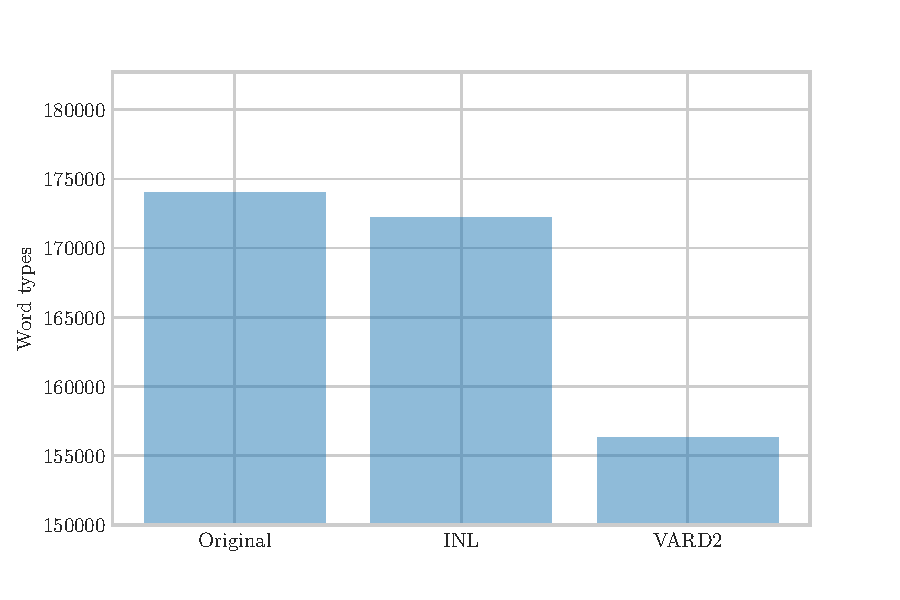
\includegraphics[scale=0.9]{Effect_normalization}
	\caption{Effect of normalization on number of word types}
	\label{fig:NormWordtypes}
\end{figure}

\section{VARD2}
A more reliable tool seems the semi-automatic tool VARiant Detector (VARD), in 2005 introduced by Alistair Baron and Paul Rayson. The tool uses two lists (a normalized word list and a variant list) to suggest or replace variant words with their normalized counterparts. VARD \textit{(i)} reads a given text, \textit{(ii)} distinguishes variants within the text, \textit{(iii)} chooses the most appropriate normalized form for each variant found and \textit{(iv)} matches the variant with the normalized form.\autocite{archer_guidelines_2015} This first version of the tool used a manually created list of variants to modern equivalent mappings in order to search for and replace any spelling variants found within a text. However, it was impossible to include all possible spelling variants in a pre-defined list and therefore the tool was not of use when dealing with spelling variations in other languages than Early Modern English. Therefore, a more recent version of the tool, VARD2, was developed with a more flexible approach which allows the tool to deal with a much larger variety of spelling variants. The normalization suggestions are given, based on a combination of four different methods: \textit{(i)} known variant replacements, \textit{(ii)} character edit distance, \textit{(iii)} letter rules and \textit{(iv)} phonetic distance. \autocite{baron_vard_nodate}

In this thesis I use a setup of VARD2 that is trained to perform spelling normalization on Dutch historical texts. It was built by Ivan Kisjes and Tessa Wijckmans, as a result of a collaboration between the CREATE-project of the University of Amsterdam and the Dutch digital research platform \textit{Nederlab}. Kisjes and Wijckmans presented the setup in a paper titled \enquote{Adapting a Spelling Normalization Tool Designed for English to 17th Century Dutch} during the Digital Humanities Conference in Mexico City in 2018.\autocite{kisjes_adapting_2018} Kisjes and Wijckmans created a Dutch configuration of VARD2, using the modifiable parts of VARD2: the letter rules, the variant list and the normalized word list. As a training set they used the 1657 edition of the Dutch translation of the Bible. There were two important reasons for this choice: first, there was a modern translation of the bible available that stuck rather closely to the original word order, and second, since there was another edition of the bible printed in 1637 available, it would be possible to easily find more spelling variants for the words they had manually respelled or checked in the 1637 edition.

In the VARD2 tool it is possible to manually process a single text as well as to process a big corpus of texts. Words of texts are placed either manually or automatically into one of the following three categories: \textit{variants}, \textit{non variants} and \textit{normalized words}. VARD2 adds words to the variant category when they are not found in its real word list. Moreover, the user can add words to this category manually as well. The variant category contains all words which the system considers necessary to normalize. The normalized category contains all words which have been normalized by the user or through automatic processing. The non variants category contains all words which are in the modern lexicon. Besides the option to processing a single text, VARD2 also offers the opportunity to process a batch of texts. In that case, the manual normalization option is not available, only the automatic normalization option.

\begin{table}[]
	\centering
	\begin{tabular}{lllll}
		\toprule
		Threshold (\%) & Variants & Variants (\%) & Normalized & Normalized (\%) \\ \midrule
		30             & 122      & 12.18         & 345        & 34.43           \\
		40             & 122      & 12.18         & 345        & 34.43           \\
		50             & 123      & 12.28         & 344        & 34.33           \\
		60             & 144      & 14.37         & 323        & 32.24           \\
		70             & 152      & 15.17         & 315        & 31.44           \\
		80             & 219      & 21.86         & 248        & 24.75           \\
		90             & 263      & 26.25         & 204        & 20.36   \\  
		\bottomrule     
	\end{tabular}
	\caption{VARD2-results at different thresholds (\texttt{id} = 11218, number of tokens = 467, number of non variants = 535)}
	\label{table:VardTresholds}
\end{table}

VARD2 will generally find numerous potential normalizations for a given variant. Each of these suggestions is given a confidence score. In the case of automatic processing, the suggested normalization with the highest confidence score is used to replace each variant. However, if the system's normalization methods \enquote{struggle} with a particular variant, the highest confidence score may be relatively low -- in these cases a threshold is required, which is the minimum confidence score needed for a normalization to take place. If the threshold is not met by the top normalization suggestion, the word is left as a variant. To get a feel for a suitable threshold for my corpus, I used a single text of my corpus and checked which number of words were normalized at different thresholds. A higher threshold will increase precision (less variants will be normalized) but reduce recall. In Table~\ref{table:VardTresholds} the results are shown for different thresholds when processing one particular song (id = 11218).\footnote{I chose this song because it has a high number of word types.} These results show that there is hardly any difference between a threshold of 30\% and 50\%. The higher the threshold, the less variants are normalized. Since I observed that the tool didn't perform any wrong normalizations, I decided to set the threshold rather low, at 50\%. The above mentioned song contains the following lyrics after normalization with VARD2:

\begin{quote}
	Daar de gulde zon en maan\\
	En de mindre hemelvieren,\\
	Die het stargewelf versieren,\\
	Gods geboden gadeslaan:\\
	Daar de felle noordewinden\\
	In het bruissend element\\
	Op die stem zig laten binden:\\
	Wie roept dat hij God niet kent?\\
	
	Het aards gezinde en dwaze rot\\
	Op het vroom geslagt verbolgen\\
	En geneigd zijn lust te volgen,\\
	Durft zig uiten, daar des geen God.\\
	Welkers oordeel sta te vrezen\\
	Als het lighaam zinkt in het graf.\\
	Want de ziel verliest haar wezen,\\
	Als wij leggen het leven af.\\
	
	Aartsverraders schrikt, ziet toe\\
	Gods geduld, en hand te tergen.\\
	Voor zijn oog is geen verbergen.\\
	Vreest, vreest des Hemels strenge roe!\\
	Eenmaal zal de dag genaken.\\
	(Is zijn wrake traag in het gaan)\\
	Die u zal te schande maken,\\
	En door blixemvuur verslaan.\\
\end{quote}

\noindent Most of the wrong normalizations that the INL tool performed, are not made by the VARD2 tool: \enquote{gulde} and \enquote{zig} stay the same, as well as the verbal forms. The words \enquote{vercieren} and \enquote{hy} are correctly changed into \enquote{versieren} and \enquote{hij}. Besides that, the VARD2-tool replaces \enquote{'t} with \enquote{het}. Although in this example less words are substituted with the VARD2- tool, Figure~\ref{fig:NormWordtypes} shows that, after normalization with VARD2, the number of unique words in the corpus was reduced with 17,692, which is 10\% of the total number of unique words. This suggests that the VARD2 tool obtains better results than the INL tool, but the topic modeling results should give more insight in this case.